%Общий объем раздела 20-30 стр.

\section{Анализ предметной области. Обзор известных работ в области стегоанализа}

\subsection{Базовые понятия и положения стеганографии}

\textit{Стеганография} (от греч. στεγανός — скрытый и γράφω — пишу; буквально «тайнопись») — это наука о передаче (хранении) информации с сохранением в тайне самого факта передачи (хранения). Большинство способов классической цифровой стеганографии базируется на особенностях восприятия информации человеком, организуя сокрытие секретных сообщений таким образом, что чувствительность человеческих органов не позволяет определить их наличие.

Основными понятиями стеганографии являются понятия контейнера, сообщения и ключа. Ниже приведены их определения, данные в монографии~\cite{Agranovskiy}.

\textit{Контейнером} $ b $ ($ b \in B $, где $ B $ — множество всех возможных контейнеров) называют несекретные данные, используемые для сокрытия сообщений. В цифровой стеганографии роль контейнеров играют растровые графические изображения, цифровой звук, а также текстовые и другие электронные документы.

\textit{Сообщением} $ m $ ($ m \in M $, где $ M $ — множество всех возможных сообщений) называют секретную информацию, скрываемую в контейнере.

\textit{Ключом} $ k $ ($ k \in K $, где $ K $ — множество всех возможных секретных ключей) называют секретную информацию, известную только санкционированному пользователю стеганосистемы, которая определяет конкретный способ сокрытия и извлечения сообщения. В широком смысле ключ — это неизвестный противнику способ (алгоритм) сокрытия информации, в узком — параметр заранее оговорённого стеганографического алгоритма, без знания которого извлечение сообщения невозможно.

Общая схема стеганографической системы приведена на рис. 1.1. Согласно ей, на передающей стороне сообщение скрывается в контейнере при помощи прямого стеганографического преобразования. Затем полученный модифицированный контейнер по открытому каналу связи отправляется принимающей стороне, где при помощи обратного стеганографического преобразования извлекается исходное сообщение.

% Рисунок 1.1 -- Обобщённая схема стеганографической системы
\begin{figure}
\centering
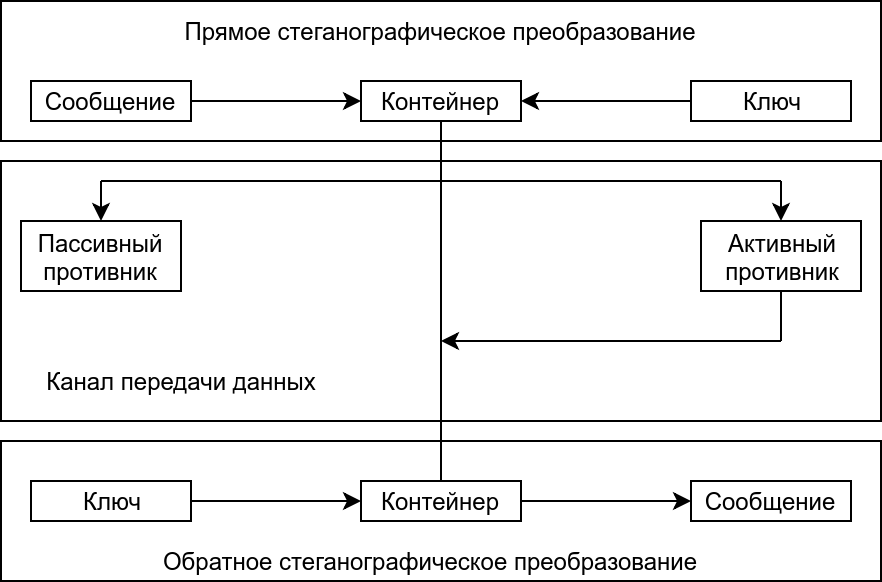
\includegraphics[width=1\textwidth]{include/graphics/im_1-stego_system}
\caption{Обобщённая схема стеганографической системы}
\label{fig:StegoSystem}
\end{figure}

Задача \textit{пассивного противника} состоит в определении факта наличия в контейнере сокрытых данных. \textit{Активный противник} пытается вносить изменения в контейнер или, в простейшем случае, уничтожить передаваемое сообщение. Решением вышеприведённых задач занимается стегоанализ.

\subsection{Основные принципы и подходы стегоанализа}

\textit{Стегоанализ} — это наука о выявлении факта передачи скрытой информации в анализируемых данных и её извлечении.

В зависимости от наличия априорных знаний о стегосистеме, задействованной для стеговстраивания, применяются направленные или слепые методы стегоанализа. \textit{Направленные} методы стегоанализа предназначены для выявления присутствия сообщения, вложенного известным стегоаналитику методом. В случае отсутствия данных о стегоалгоритме встраивания используют методы \textit{слепого} стегоанализа.

Следующий критерий классификации стегоаналитических методов — используемый подход. В зависимости от подхода можно выделить визуальные, сигнатурные, схемные и статистические методы. Рассмотрим их применительно к стегоанализу цифровых неподвижных изображений.

\textbf{Визуальные методы} основаны на способностях зрительной системы человека, а именно, возможности анализировать зрительные образы и определять различия в сопоставляемых изображениях.

Такие методы стегоанализа графических файлов являются самыми простыми, так как не требуют математической и программной реализации,  но они неспособны обнаружить современные методы стеговстраивания.

Подходом \textbf{сигнатурных методов} является синтаксический анализ последовательности битов анализируемого контейнера.

В первых известных алгоритмах скрытия сообщений в цифровых изображениях заполнение контейнера производилось путём замены служебных атрибутов файла на встраиваемую информацию~\cite{FridrichBook}, что позволяло относительно просто составить сигнатуру, характеризующую заполненный стегоконтейнер, и свести задачу стегоанализа к поиску сигнатуры.

Дальнейшее усовершенствование стеганографических методов привело к широкому распространению стегосистем, осуществляющих встраивание в пространственной области изображения, но сигнатурные методы всё ещё могли противостоять таким стегосистемам. Например, в работе~\cite{HideAndSeek} описывается сигнатурный метод стегоанализа изображений в оттенках серого, обработанных с помощью программы Hide and Seek версий 4.1 и 5.0. Выходом программы являются изображения, содержащие три канала цветности с одинаковыми значениями цветовой координаты в каждом. Наиболее распространённым способом хранения трёхканальных изображений является кодирование каждой цветовой координаты 8-битным числом, определяющим диапазон уровней квантования $ q = {0,...,255} $ и шаг квантования $ h = 1 $. Hide and Seek использует $ q = {0,...,252} $ и $ h = 4 $, что позволяет выделить контейнеры, заполненные этой программой, на общем фоне.

Преимуществом данного подхода является высокая скорость работы реализующих его алгоритмов, но сильная привязка к атрибутам заполненных стегоконтейнеров, не учитывающая принципы стеговстраивания, является существенным недостатком, не позволяющим широко использовать данный подход.

\textbf{Схемные методы} применяются для проверки гипотез о наличии стеганографического встраивания с применением известной стегосистемы.

Основными достоинствами схемных методов являются низкая вероятность возникновения ошибок и возможность идентификации стеганографической системы с последующим извлечением сообщения.

Фатальными недостатками данного подхода являются невозможность реализовать необходимое для применения слепого стегоанализа количество стегосистем и многообразие ключей, позволяющее стегосистеме существенно менять характер стеговстраивания от одного ключа к другому.

\textbf{Статистические методы} базируются на понятии «естественного» контейнера. Их суть заключается в оценивании вероятности существования стегосообщения, встроенного неизвестной стегосистемой на основе критерия близости исследуемого контейнера к «естественному» путём обнаружении отклонения анализируемой информации от ожидаемой модели.

Преимуществом подхода является возможность применения в слепом стегоанализе, недостатком — высокая сложность создания модели «естественного» контейнера.

\subsection{Известные методы стегоанализа на основе статистической обработки данных}
\subsection{Применение глубоких искусственных нейронных сетей в задачах стегоанализа}
\subsubsection{Свёрточная нейронная сеть GNCNN}

Модель свёрточной нейронной сети для стегоанализа изображений в оттенках серого GNCNN была предложена в~\cite{GNCNN}. Её основные отличительные особенности: применение фильтра предварительной обработки и использование функции Гаусса в качестве функции активации нейронов свёрточных слоёв.

\begin{equation}
\label{eq:GNCNNConvKernel}
%\begin{align*}
K = \frac{1}{12}
\begin{pmatrix*}[r]
    -1 &  2 &    -2 &  2 & -1 \\
     2 & -6 &     8 & -6 &  2 \\
    -2 &  8 & -12 &  8 & -2 \\
     2 & -6 &     8 & -6 &  2 \\
    -1 &  2 &    -2 &  2 & -1 \\
\end{pmatrix*}
%\end{align*}
\end{equation}

Полосовой высокочастотный фильтр предварительной обработки с импульсной характеристикой~\eqref{eq:GNCNNConvKernel} введён исходя из априорного знания о слабом характере стеговоздействия на стегоконтейнер. Целью предварительной фильтрации является усиление яркости стегосигнала и ослабление яркости оригинального изображения. Веса данного фильтра заранее предопределены и не участвуют в процессе обучения нейронной сети.

Ещё одним преобразованием, облегчающим процесс извлечения признаков, является переход от оригинального изображения к шумоподобному остатку $ R = (r_{ij}) $, содержащему только предсказания относительно факта стеганографической модификации каждого пикселя:

\begin{align*}
r_{ij} = y_{ij} - P(N(Y, i, j)),
\end{align*}

где $ Y = (y_{ij}) $ – стегоконтейнер, а $ P(N(Y, i, j)) $ – оценка значения пикселя $ y_{ij} $, полученная из окружающих его пикселей $ N(Y, i, j) $~\cite{FridrichNoiseResidual}. Ввиду наличия сложных зависимостей между соседними пикселями, в случае отсутствия модификации оценка зачастую будет близка к действительному значению пикселя $ y_{ij} $, а значение $ r_{ij} $ будет близко к нулю.

\begin{equation}
\label{eq:GaussianFunction}
%\begin{align*}
f(x) = e^{-\frac{x^2}{\sigma^2}}
%\end{align*}
\end{equation}

Функция Гаусса~\eqref{eq:GaussianFunction} с нулевым математическим ожиданием в качестве функции активации (рис.~\ref{fig:GaussianFunction}) призвана обеспечить формирование в свёрточном слое нейронной сети такого ядра $ K $, что $ Y*K = R $. Максимальное значение функции в нуле соответствует нулевой ошибке оценки значения $ y_{ij} $ и, следовательно, предположению об отсутствии модификации пикселя стегоконтейнера. Резкий спад по мере удаления от нуля обращает в близкие к нулю значения любой результат свёртки, превышающий порог, определяемый среднеквадратическим отклонением $ \sigma $, влияющим на ширину кривой. В рамках эксперимента использовалось значение $ \sigma = 0,1 $.

% Рисунок 1.2 -- Gaussian function
\begin{figure}
\centering
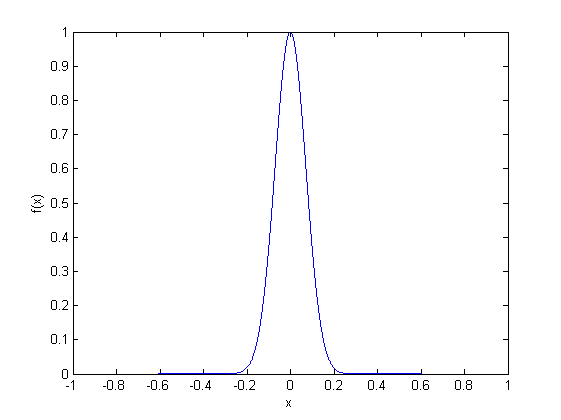
\includegraphics[width=1\textwidth]{include/graphics/im_2-gaussian_function}
\caption{Функция активации GNCNN}
\label{fig:GaussianFunction}
\end{figure}

В процессе обучения в качестве функции потерь применялась категориальная кросс-энтропия. Используемый метод обучения – Adam со скоростью обучения 0,001, $ \beta_1 = 0,9 $, $ \beta_2 = 0,999 $. Архитектура нейронной сети представлена на рис.~\ref{fig:GNCNNArchitecture} и имеет вид состояний, через которые проходит входное изображение.

% Рисунок 1.3 -- GNCNN Architecture
\begin{figure}
\centering
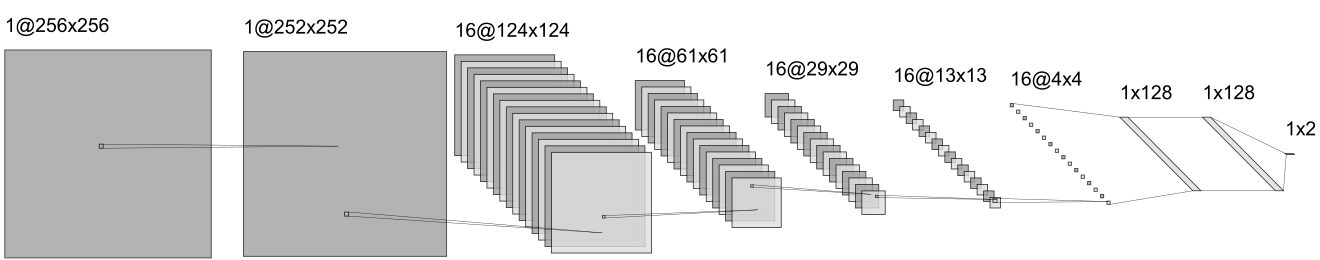
\includegraphics[width=1\textwidth]{include/graphics/im_3-gncnn_architecture}
\caption{Архитектура GNCNN}
\label{fig:GNCNNArchitecture}
\end{figure}

На вход нейронной сети подаётся изображение в оттенках серого в разрешении 256×256 пикселей. Фильтр предварительной обработки с ядром~\eqref{eq:GNCNNConvKernel} является первым свёрточным слоем и в обучении не участвует. За ним следуют пять свёрточных слоёв, состоящих из 16 каналов. Каждый из них осуществляет операцию свёртки с ядром, формирующимся по мере обучения сети, а также вычисление функции активации и выполнение субдискретизации по среднему с размером окна 3×3 и шагом 2. Первые четыре обучаемых слоя используют ядра размера 3×3, последний – 5×5.

Выход последнего свёрточного слоя представляет собой 256 выделенных признака. Они помещаются в модуль классификации, состоящий из трёх полносвязных слоёв: первые два имеют по 128 нейронов каждый и функцию активации ReLU, последний – два нейрона и функцию активации softmax.

\subsubsection{Нейронная сеть с двумя свёрточными слоями}
Также в рамках работы была рассмотрена свёрточная нейронная сеть для стегоанализа изображений в оттенках серого, предложенная в~\cite{FrenchCNN}. Для корректности эксперимента размеры слоёв были изменены для работы со входными изображениями в разрешении 256×256 пикселей. Архитектура нейронной сети приведена на~\ref{fig:FrenchCNNArchitecture}.

% Рисунок 1.4 -- French CNN Architecture
\begin{figure}[!htb]
\centering
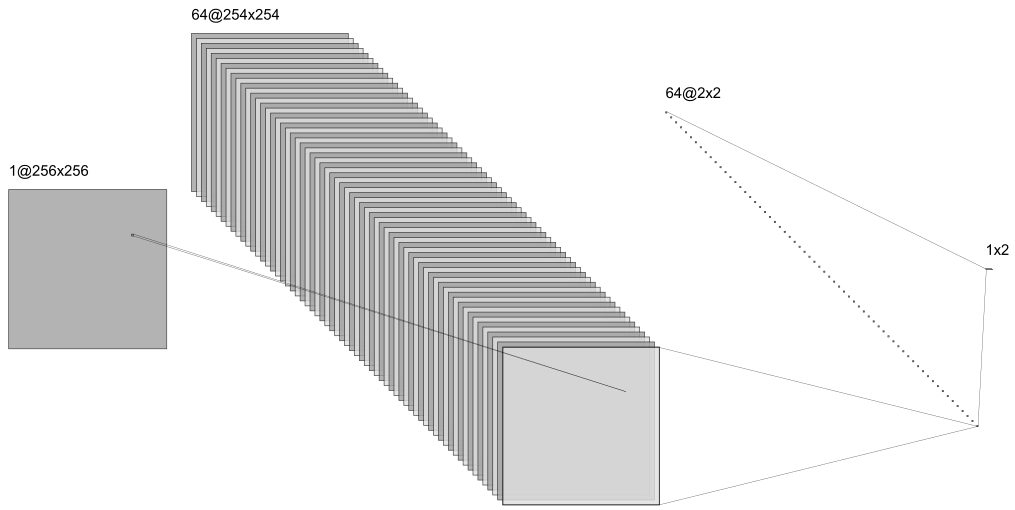
\includegraphics[width=1\textwidth]{include/graphics/im_4-french_cnn_architecture}
\caption{Архитектура сети с двумя свёрточными слоями}
\label{fig:FrenchCNNArchitecture}
\end{figure}

На вход нейронной сети подаётся изображение в оттенках серого в разрешении 256×256 пикселей. Первый свёрточный слой имеет размер 3×3, за ним следует свёрточный слой размера 253×253, состоящий из 64 каналов. Оба свёрточных слоя осуществляют операцию свёртки с обучаемым ядром и вычисление функции активации tanh. Результатом их работы являются 64 карты признаков размера 2×2, соединённые с двумя нейронами с функцией активации softmax.

В качестве функции потерь была использована категориальная кросс-энтропия, метод обучения – стохастический градиентный спуск со скоростью обучения 0,005.
\clearpage